\section{Evaluation} \label{section:evaluation}

Here we present the evaluation of a distributed CQBS broker.
All brokers and coordinators machines were chosen to emulate commodity hardware; for CQBS to be an effective solution, it must not rely on intractably large resources.
Hence, we chose to use the \texttt{t2.medium} AWS instance type with 2 vCPUs and 4 GB RAM, running Ubuntu 14.04.
As we will demonstrate below, the CQBS system is amenable to commodity systems because its performance is limited by the serialization of the etcd log, and not by memory, CPU, disk, or network bandwidth.

\subsection{Performance}

\begin{figure}[t]
\centering
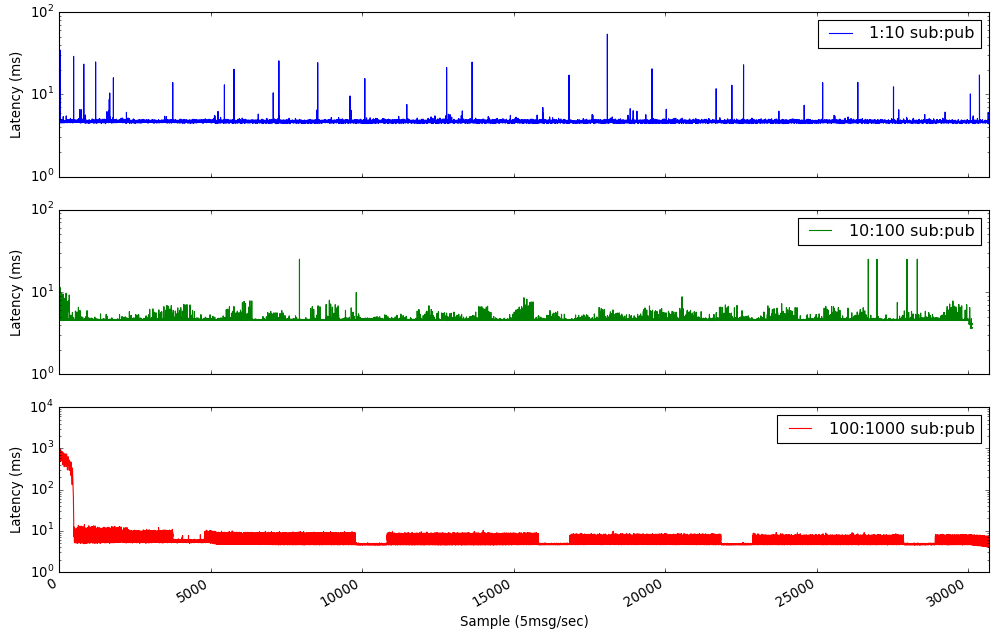
\includegraphics[width=\linewidth]{figs/singlenodelatency.png}
\caption{Microbenchmark: standalone CQBS broker forwarding latency with increasing concurrency}
\label{fig:singlenodelatency}
\end{figure}

\begin{figure}[t]
\centering
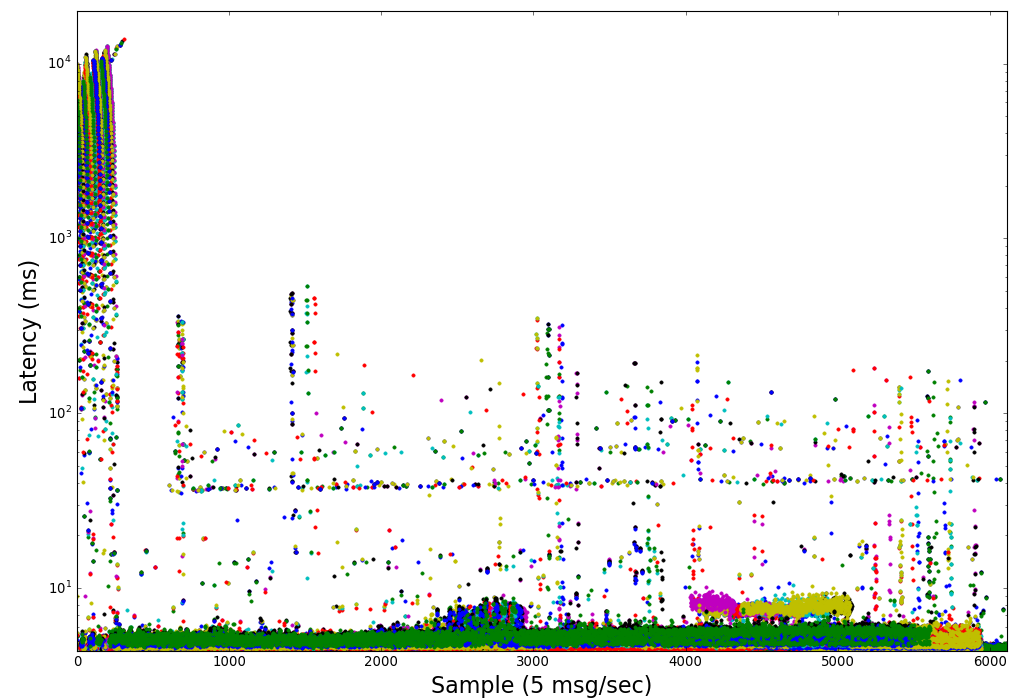
\includegraphics[width=\linewidth]{figs/fullsystem_metadatachange.png}
\caption{Benchmark: forwarding latency with 30 subscribers, 360 publishers in a 3 broker, 3 coordinator system. Each publisher changes metadata every 30-60 seconds, causing the broker to reevaluate roughly a third of all subscriptions every few seconds.}
\label{fig:fullsystem_metadatachange}
\end{figure}


\textbf{Single Broker Latency Microbenchmark:} First, we examine the latencies of the CQBS broker's forwarding mechanism in isolation -- without the communication overhead imposed by the fully replicated system.
We run a single broker on a \texttt{t2.medium} instance, backed by MongoDB.
Using a ratio of 10 publishers to one subscriber, we run three benchmarks with 1, 10 and 100 subscribers (with 10, 100 and 1,000 publishers accordingly).
Each publisher sends 5 messages per second; after the initial registration message (the high latencies at the beginning of each benchmark), each publisher sends only its stream UUID and an increasing counter as its value.
Each group of publishers/subscribers use entirely isolated sets of keys, so that they do not explicitly interfere with each other in the broker.
These three microbenchmarks are shown in Figure~\ref{fig:singlenodelatency}, and demonstrate that the latency is fairly consistent as the amount of concurrency scales.

The spikes in latency seen in the $N=1,10$ graphs are due to the pauses enacted by Go's garbage collection.
Fortunately, these do not affect the vast majority of requests.
For the $N=1,10$ cases, the mean latencies, 95\textsuperscript{th} percentile latencies and standard deviation are $4.67ms/4.85ms/0.55ms$ and $4.62ms/4.77ms/0.37ms$ respectively.
For the $N=100$ case, the garbage collection becomes more visible in the variability of response times, with mean, 95\textsuperscript{th} percentile and standard deviation latencies of $13.58ms/8.87ms/67.13ms$.
The troughs in the $N=100$ case are an odd phenomenon, most likely caused by garbage collection in the single Go process used to generate the 100 subscribers and 1000 publishers, generating approximately 5000 messages per second.

The microbenchmark demonstrates that a single broker can quite easily handle a constant load of publishers and subscribers with low latency, even on commodity hardware.

\textbf{Full System Query Reevaluation Overhead}: To evaluate the overhead of the continuous syndication mechanism, we construct three broker, three coordinator cluster, with every component running on a different machine.
We then introduce 10 subscribers at every broker; each subscribes to 4 local publishers (same broker) and 4 remote publishers at each of the other two brokers for a total of 12 subscriptions.
In total, there are 120 publishers per broker, with a total of 30 subscribers and 360 publishers in the benchmark.
Each publisher changes its metadata every 30-60 seconds, causing the publishers to cycle among the subscribers.
The results are illustrated in Figure~\ref{fig:fullsystem_metadatachange}, which illustrates the limitations of serializing the processing of all metadata changes and coordinator updates.
While the 95\textsuperscript{th} percentile latency is only $7.59ms$, the mean latency over the experiment was $129.60ms$ with a standard deviation of $891ms$.
This variability is caused when several metadata updates arrive at the coordinator in quick succession: the coordinator buffers these changes until it can process them sequentially, making sure that the forwarding tables are correct and consistent.
Because no related messages can be forwarded until the forwarding changes are known, a queue of metadata changes causes cascading delays until the system can catch up.
This phenomenon is most prominent around samples 800, 1500, 3000 and 4000.
The ``waterfall'' at the beginning of the stream is caused by all 30 subscribers and 360 publishers querying and registering at the same time, placing a large load on MongoDB and the etcd log.

When considered in conjunction with the microbenchmark above, it is clear that the serialization of the metadata changes and coordinator updates is the limiting factor in system performance.
However, in the authors' experience with real world sensor systems using similar systems, these high rates of change are rarely seen: it is important to note that these loads are intentionally heavy to find the bottlenecks in the system.

\subsection{Client Complexity}

\subsection{Fault Tolerance}
